\chapter{Analysis and Results}


\section{2022 vdM scan program}

In November 2022, the main vdM scan program for the CMS experiment was conducted during LHC fills 8379 and 8381 on 10 and 11 November of 2022. During fill 8381, a total of 144 bunch pairs were colliding at the CMS interaction points at zero crossing angle, with a proton-proton collision energy $\sqrt{s}$ of 13.6 TeV. 
During this fill, various types of scan pairs with different characteristics were conducted. These scan pairs are described below. Each scan pair consisted of two scans in the transverse planes $x$ and $y$. In addition to these scans, other types of scans were also conducted, which are not included in this analysis.\\ %explicar porque se colisionan solo 144 de 2500 bunches en fisica

The calibration program included four scan pairs, vdM1,vdM2, vdM3 and vdM4, these are considered the standard vdM scans in the program and they are used only for the main calibration, in this type of scan the two beams are separated by $6\sigma_{b} \thickapprox 578\mu m$, where $\sigma_{b}$ represents the transverse bunch size. The beams are then scanned across each other in a sequence of 25 steps, each lasting 30 seconds with a step size of $0.5\sigma_{b} \thickapprox 48 \mu m$.\\

The calibration program also included two beam-imaging scan pairs, BI1 and BI2 . These sscans were used for main analysis and also for studies on beam shapes,correcting the effects caused by the not strictly valid assumption that the bunch proton density function is factorizable into independent $x$ and $y$ densitys ($x$-$y$ nonfactorization). During the BI scans, one beam is kept fixed at its nominal head-on position, while the other beam is separated and scanned in 19 steps. Each step lasts 46 seconds and covers a range from $-4.5\sigma_{b}$ to $+4.5\sigma_{b} \thickapprox 433 \mu m$.\\
% can lead to a biased estimate of the beam overlap area.  (x-y nonfactorization), 

Two length scale LS scans were conducted, one during fill 8381 and another during fill 8379. The LS scan is a special scan designed to apply a correction to the results obtained from the vdM scan program. During this scan, the beams are separated by a constant amount of $\sqrt{2} \sigma_{b} \thickapprox 106 \mu m$, and they are moved coherently forward and backward in five steps each, all in the same transverse direction.\\

Finally two super separation periods SS1 and SS2 were performed for the Background esimation, here the two beams were sepated at a distance of $6\sigma_{b}$ during 5 minutes.
%23:31-23:36 11:47-11:52

The scan program during fill 8381 is summarized in Figure \ref{scan_prog} where all the scans mentioned and described above are labeled.

\begin{center}
  \begin{figure}[h]	
    \centering
    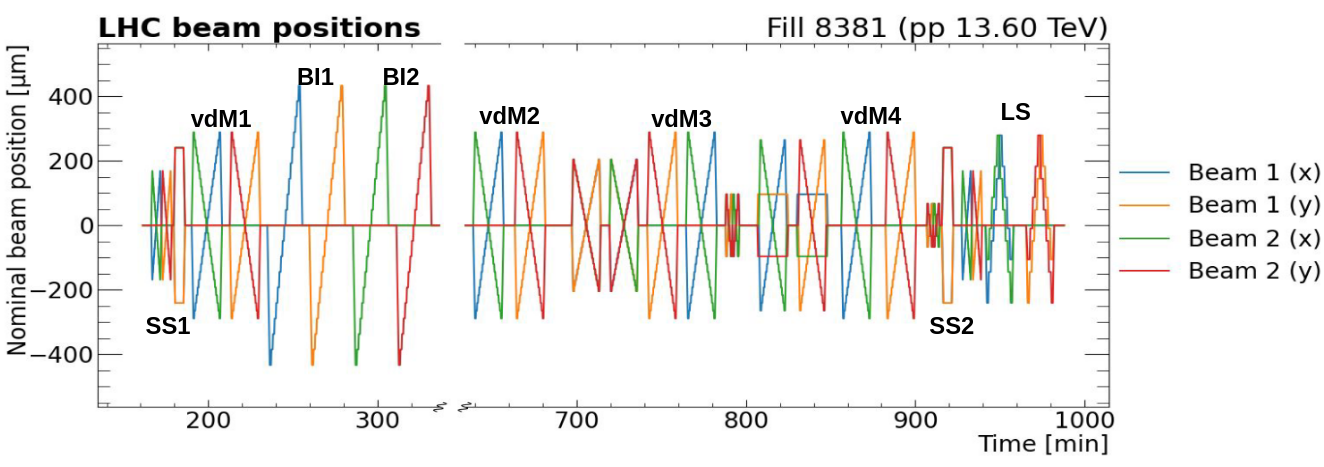
\includegraphics[scale=.35]{Chapter4/2022Scanprorgam.png}
    \caption[2022 scan program]{Nominal horizontal and vertical positions of the proton beams during LHC fill 8381, showing the four standard vdM scans, two BI scans, one LS scan and the two Super Separation Periods (SS)}
    \label{scan_prog}
  \end{figure}
\end{center}

\section{Data aquisition and processing}

In order to achieve a high statistical precision in data for each  bunch pairs BCID, the system trigger  bandwidth  limitations do not allow the use of all BCID's, beacause this, CMS implemented a zero bias triggers only on five BCID's: 282, 822, 2944, 3123, and 3302. This data is saved randomly with the highest possible rate of 27.23 kHz using the High Level Trigger system (HLT)  through the data acquisition (DAQ) system. Due to the weight of the events, 16 different streams are required to save the full data. Here the datasets are in their called RAW version.\\

The data is then reprocessed by the CMS collaboration to enable a cluster reconstruction, resulting in the datasets (ALCARECO version) that contain the number of clusters per event and all their additional information, the data here is in the CMSSW format. These datasets will be used as the starting point for our own data reprocessing and analysis.\\

To begin our analysis, we extracted the all the necessary information from the datasets using the CMS software , which is written in Python and C++. Due to the large size of the datasets, all the datasets were sent for reprocessing through The Worldwide LHC Computing Grid (WLCG), wish consists of a grid-based computer network infrastructure,designed by CERN to handle the big volume of data produced by LHC experiments.\\
After processing, we obtained the required event-level information, which was saved in a dataset with a ROOT format. This format uses Trees and Branches, that are containers to maintain the information in a hierarchical and organized manner. The information stored in one of these containers includes general information such as the number of run, the number of lumisections (where 1 LS = 23 s), and the number of luminible LN (where 1 LN is equivalent to 0.32 s). In another container, we can find the number of clusters per event, the bunch number "BCID" of the event, the event timestamp, and the module identifiers of the event. \\
  
Due to the limitations of the framework for handling our size of data, we are unable to use all of the statistics as we have them. To address this issue, we need to merge the data in a single file with a hierarchical data format (hd5) that saves the information organized in tables. In order  to utilize all the statistics in this only file,we stored  the rates each 1.32 s (NB4) time that corresponding to 4 LN, this is an average  between clusters and the number of events that fall within this time span. Again the process is done by the WLCG. During this reprocessing phase, the veto list is introduced, and the detected events in these modules are eliminated.\\

The final hd5 file, containing the rates collected during the vdM scans, is analyzed using the vdM Framework (vdMFW), which is written in Python and uses the ROOT data analysis package through the PyRoot library. The vdMFW reads the hd5 file and extracts the necessary information for analysis using its analysis tools. During the analysis process, several corrections are applied to the rates which will be described later.
After the complete analysis, the Framework generates the final information and plots, which contain the normalized rates ($R/N_{1}N_{2}$) and beam position.  A mathematical function is then used to fit the points to extract $\Sigma_{x,y}$ and peak values to compute $\sigma_{\text{vis}}$ for all the bunches in the scan.

\section{Background estimation}

To extract $\Sigma_{x,y}$ through fitting, it is necessary to correct the raw measured rates for background in the detector beforehand. The background contribution is estimated independently during the Super Separation (SS) period comented in the above section. There are three principal sources of beam-induced background to consider:
%During this period, the beams are separated by $6\sigma_{b}$, ensuring that the only contribution is from background.
\begin{itemize}

\item Beam Gas Elastic (BGE). The elastic beam gas contribution are all coherent and quasi-elastic, nuclear elastic and coulomb scattering for multi-turn beam-gas interactions around the ring. Typically the interaction of the primary beam proton and the takes place at the tertiary TCT collimator jaw \cite{bkg_source}.
%%citar
\item Beam Gas Inelastic (BGI). These are all inelastic interactions of primary beam protons with rest gas in the beam pipe. The interaction rate is dominated by the vacuum quality in the various beam line elements upstream CMS. Therefore the origin of this contribution is distributed all along the long straight section \cite{bkg_source}.

\item Beam Halo (BH). This component of the machine induced background is caused by the inefficiency of the main collimation system. Protons can escape from one collimator and being intercepted by another collimator \cite{bkg_source}.
\end{itemize}

In order to illustrate the two SS periods for this analisys, Figure \ref{ssp_wide_bx282} displays the PCC per NB4 versus time for BCID 282. The lower regions of the plot correspond to a time window of 5 minutes during which the beams were separated by a distance of $6\sigma_{b}$.\\

\begin{center}
\begin{figure}[h!]
\centering
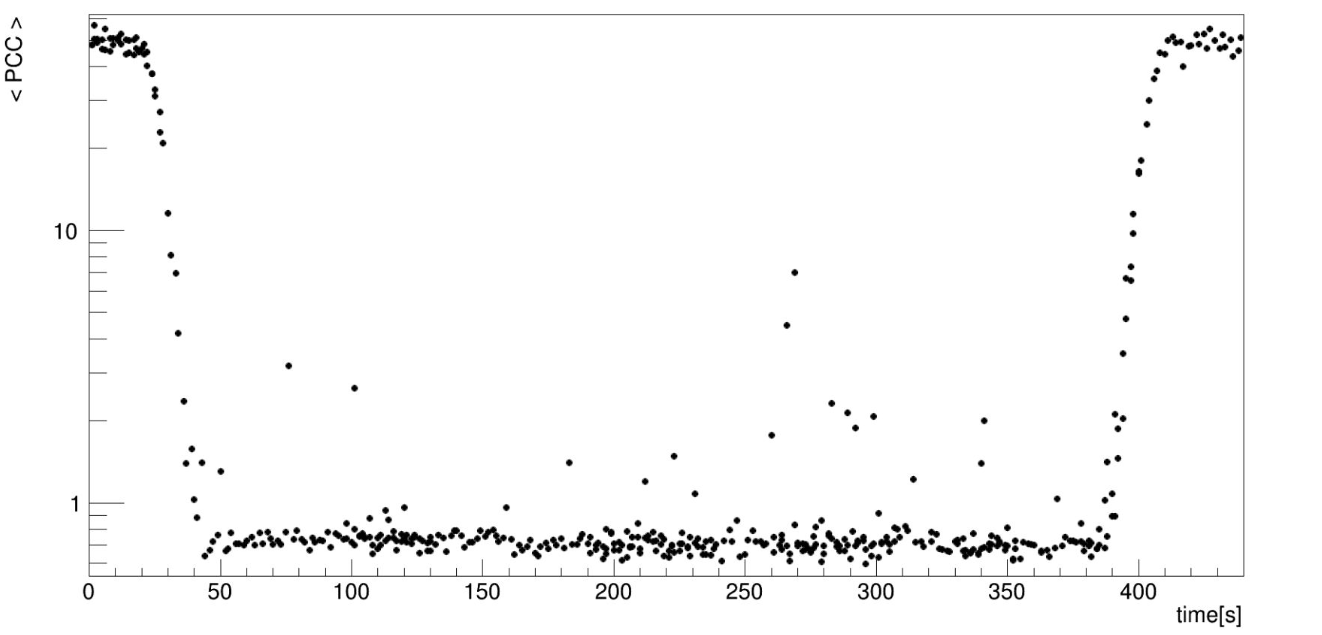
\includegraphics[width=.49\textwidth]{Chapter4/BX_282_Rates_SS1.png}
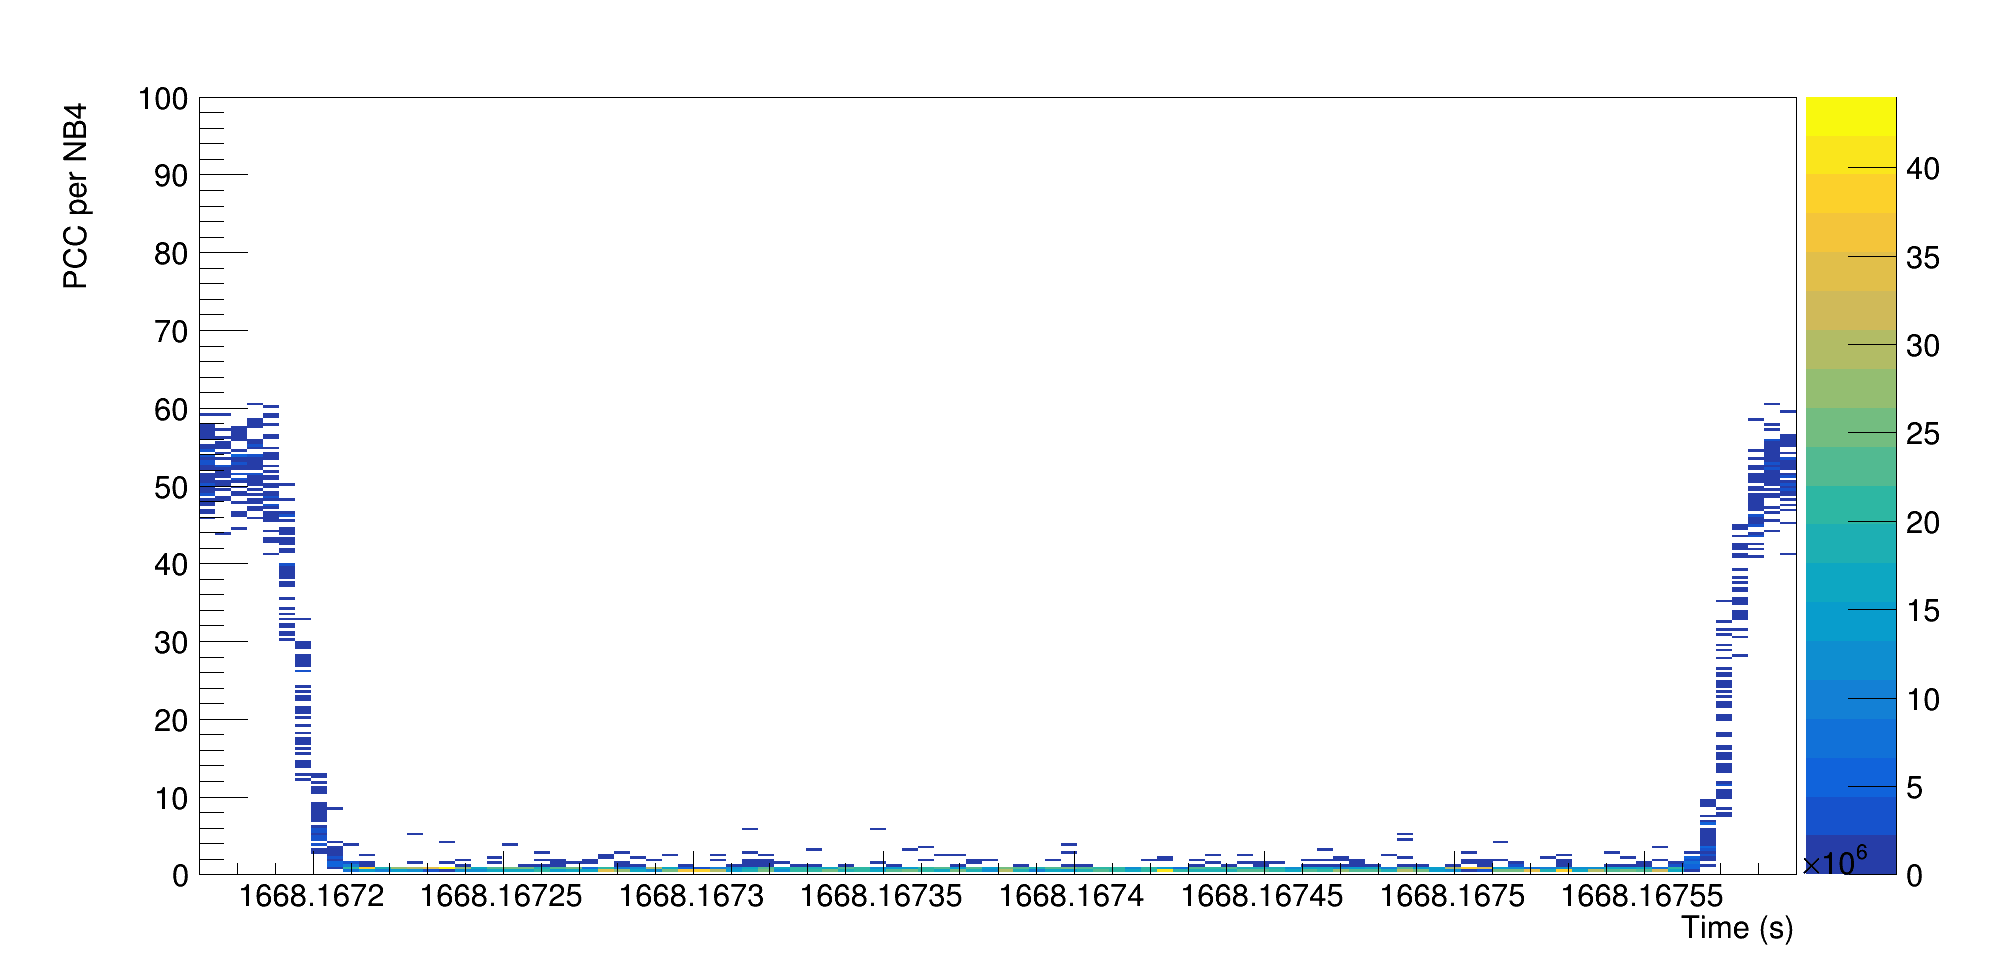
\includegraphics[width=.49\textwidth]{Chapter4/BX_282_Rates_SS2.png}
\caption[Super Separation periods for BCID 282]{PCC per NB4 versus time for BCID 282. The lower regions corresponds to the super separation period I (left) and II (right).}
\label{ssp_wide_bx282}
\end{figure}
\end{center}

To estimate the background value in each BCID, the mean value of the PCC per NB4 rates distribution is computed. The mean and error per super separation (SS) period are obtained by plotting the PCC per NB4 as a function of time and then taking the $y$ projection. The error is calculated using the formula $AvgErr = \sqrt{SEM_1^2 + SEM_2^2 + \cdots + SEM_N}/N$. To illustrate this process for each BCID, the distribution or profile of PCC per NB4 for each SS period is plotted. Figure \ref{ss1_hist_282} displays the PCC per NB4 distribution for SS period I specifically for BCID 282, but the same plot is created for every BCID.\\

\begin{center}
  \begin{figure}[h!]
    \centering
    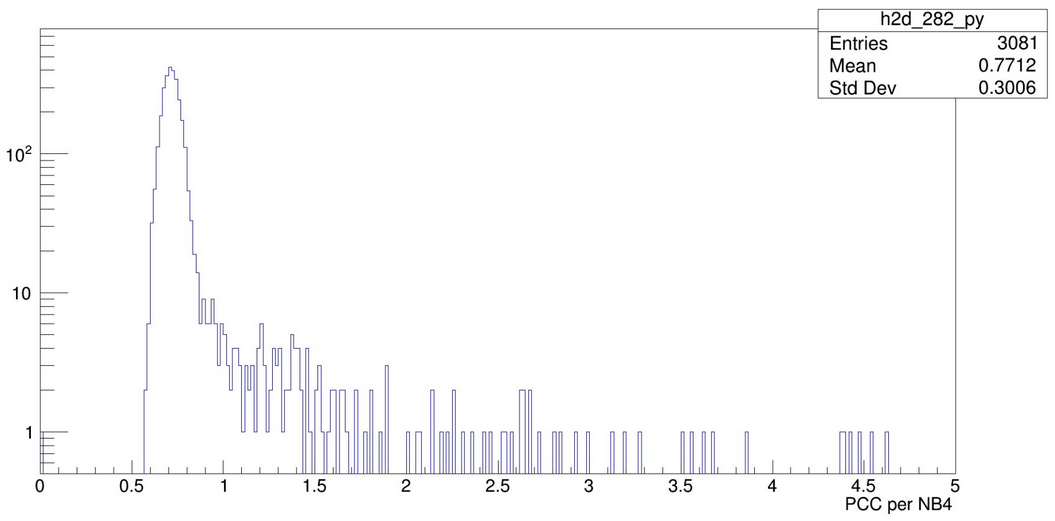
\includegraphics[scale=.18]{Chapter4/ss1_histo_bx282.png}
    \caption[PCC per NB4 profile for BCID 282 from SS period I]{ PCC per NB4 profile for BCID 282 from SS period I.} 
    \label{ss1_hist_282}
  \end{figure}
\end{center}


\begin{table}[h!]
  \begin{center}
    \caption{Mean and standard error on mean (SEM) for the PCC background estimated with the SS1 and SS2 data, separately for all five BCIDs and averaged.}
    \label{ss_per_bx}
    \begin{tabular}{|c | c | c | }
      \multicolumn{1}{c}{} & \multicolumn{1}{c}{\textbf{SS period I}} & \multicolumn{1}{c}{}  \\
      \hline
 \textbf{BCID}   & \textbf{Mean}   &  \textbf{SEM}\\
     \hline %\midrule[1.1pt]
      282 & 0.7712 & 0.0054\\
      \hline
      822 & 0.7744 & 0.0055\\ 
      \hline
      2944 & 0.7695 & 0.0057\\ 
      \hline
      3123 & 0.7469 & 0.0049\\ 
      \hline
      3302 & 0.7708 & 0.0049\\ 
      \hline
      \multicolumn{1}{c}{} & \multicolumn{1}{c}{} & \multicolumn{1}{c}{}\\
      \multicolumn{1}{c}{$\text{SSI}_{\text{Avg}}=$} & \multicolumn{1}{l}{$0.7665 \pm 0.0023$} & \multicolumn{1}{c}{}\\
%      \multicolumn{1}{c}{} & \multicolumn{1}{c}{} & \multicolumn{1}{c}{}
    \end{tabular}
    \hspace{0.5cm}
    \begin{tabular}{|c | c | c | }
      \multicolumn{1}{c}{} & \multicolumn{1}{c}{\textbf{SS period II}} & \multicolumn{1}{c}{ }  \\
      \hline
 \textbf{BCID}   & \textbf{Mean}   &  \textbf{SEM}\\
     \hline %\midrule[1.1pt]
      282 & 0.7192 & 0.0048\\
      \hline
      822 & 0.7257 & 0.0057\\ 
      \hline
      2944 & 0.7292 & 0.0058\\ 
      \hline
      3123 & 0.7028 & 0.0052\\ 
      \hline
      3302 & 0.7208 & 0.0053\\ 
      \hline
      \multicolumn{1}{c}{} & \multicolumn{1}{c}{} & \multicolumn{1}{c}{}\\
      \multicolumn{1}{c}{$\text{SSII}_{\text{Avg}}=$} & \multicolumn{1}{l}{$ 0.7195 \pm 0.0024$} & \multicolumn{1}{c}{}
    \end{tabular}   
  \end{center}
\end{table}

Table  \ref{ss_per_bx} shows the results for five different BCIDs, using the reprocessed PCC data for Fill 8381.  The overall background correction applied to raw PCC rate is $0.74305 \pm 0.002407$, which is calculated by taking the average of the mean values of SS1 and SS2. 

This analysis shows significant inconsistencies between the background values for the two SS periods, therefore it was excluded from the following analyses.

\section{Beam Corrections}

There are several systematic effects that affect the measurement of beam overlap width and therefore the extraction of $\sigma_{vis}$ from the vdM scan procedure. These effects are measured and, where applicable, corrected as described below. A systematic uncertainty is assigned to the resulting measured cross section $\sigma_{vis}$, and the following corrections are applied in the vdM Framework:
 
\begin{enumerate}

\item Ghost and Satellite. This correction corrects for the presence of spurious charges, which affect bunch currents. Satellite charges refer to additional charges outside the actual colliding bunch, while ghost charges refer to charge not in any nominally filled bunch slot. These results in corrections of up to 0.5\% to $\sigma_{vis}$. The overall uncertaintys estimate the bunch current measurement  to be 0.4\%.

\item Orbit drift. The orbit drift correction accounts for potential movement of the LHC orbit during the vdM scans. Time-dependent changes of the transverse beam positions for fixed machine parameters can alter the beam separation. This correction is composed of two independent corrections: 

\begin{itemize}

\item Orbit drift separation "ODS", correction that aims to correct for the orbit drift in the scanning direction and only affects beam separation. 

\item  Orbit drift rate "ODR", correction that aims to correct for the orbit drift in the direction orthogonal to the scanning direction and only affects the luminometer rate. The derived correction assumes that the beam overlap has a single Gaussian shape. The correction reads the $\sigma_{vis}$ in the orthogonal direction from the previous correction. 
\end{itemize}

Applying this correction improves the agreement between the $\sigma_{vis}$ values derived with different scan pairs and changes the average $\sigma_{vis}$ by about 0.3\%. The full size of the correction is considered as uncertainty.

\item Beam Beam corrections.  The electromagnetic interaction between the two colliding proton bunches leads to two effects in beam-separation scans:

\begin{itemize}

\item Beam Beam deflection. Corrects Beam Beam deflection (BB) that happens during bunch crossings at the collision point. Accounts for the electrical repulsion of the beams, which increases the lateral separation. The deflection is calculated and added to the nominal separation.

\item Dynamic Beta. The so-called dynamic $\beta^{*}$  effect, which accounts for any changes in the proton density distributions of the bunches due to the single-particle interactions. As a result, the non-linear change during separation steps in transverse bunch profiles is observed, and can described by the effective change of the $\beta^{*}$  value.
\end{itemize}
The corrections are calculated for each proton bunch pair individually, and the combined effect of the two corrections is an increase of $\sigma_{vis}$ by 1.0\%, with an uncertainty of 0.5\%.

\item Length Scale.  It applies a linear scaling to the beam separation to convert it from the "CMS scale" to the actual "physics scale". This is  calibrated by analyzing pp collision vertices reconstruced by the CMS tracker using data from the five length scale scan pairs performed in fills 8178, 8379, and 8381.This correction reduces $\sigma_{vis}$ by 1.0\% and results in an uncertainty of 0.12\%.

\end{enumerate}

\section{Model  Selection}

As we have seen in previous sections, the points generated for each step of the scan need to be fitted using a mathematical function. This allows us to extract the parameters we need, such as $\Sigma_{x,y}$ and peak values for all the bunches in the scan, in order to finally compute $\sigma_{\text{vis}}$. Within vdMFW, there are several pre-defined functions that use a combination of Gaussian functions with different adjustable parameters to achieve a better fit. These functions include Double Gaussian (DG), Single Gaussian (SG), Poly Gaussians (PG), among others. All of the above functions exist in versions with an additive constant to the entire function, typically used to fit to the background levels.\\

For this analysis, various fit functions were tested, and the one with the best quality of fit was selected. The quality of the fit is primarily based on the convergence of the function with the points being fitted for each BCID. The convergence is assessed based on the covariance matrix, which measure the linear relationship between each pair of elements or variables. A  covariance status equal to 3 means a good convergence of the function.\\ 

The second most important parameter for measuring the quality of the fit is having a good  Chi-square $\chi^2$. The  Chi-square goodness of fit test is a statistical hypothesis test that helps to determine whether a variable is likely to come from a specified distribution or not. This test provides a way to assess whether the data values have a good enough fit to our model, or if the model is questionable. In more general terms, this test compares observed values with expected or theoretical values according to the hypothesis.\\

This can be seen in figure \ref{chi2} where $N$ observed values $y_{1}$,···, $y_{N}$ are measured with errors $\sigma_{1}$,···,$\sigma_{N}$" at the values of $x$ given without error by $x_{1}$,..., $x_{N}$. The theoretical  value $\lambda_{1}$ of $y_{l}$. is given by a function $\lambda_{i} = \lambda(x_{i},\theta)$. The value of $\theta$ is adjusted to minimize the value of $\chi^2$, given by equation \ref{x^2}, where it is inferred that the lower the value of $\chi^2$, the better the fit is considered to be \cite{Statistical_Data_Analysis}.

\begin{equation}
\chi^{2}(\theta)=\sum_{i=1}^{N} \frac{(y_{i}-\lambda(x_{i},\theta))^{2}}{\sigma_{i}^{2}}
\label{x^2}
\end{equation}

\begin{center}
  \begin{figure}[h!]
    \centering
    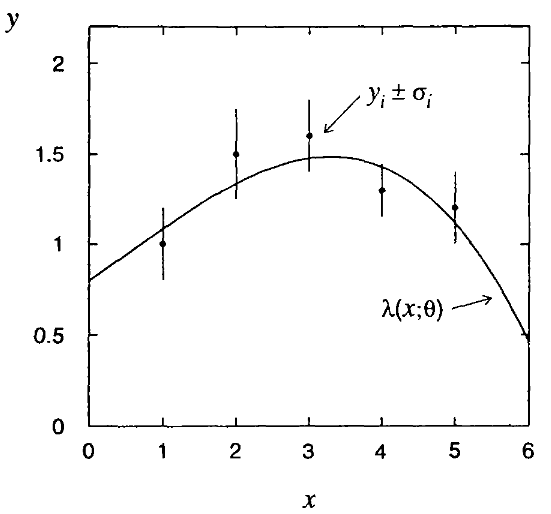
\includegraphics[scale=.35]{Chapter4/chi-square.png}
    \caption[chi-square definition]{ chi2/ndof } 
    \label{chi2}
  \end{figure}
\end{center}

\section{Results}
%In the previous section, inconsistencies were observed in the background values, which resulted in a very high chi-square value. Therefore, it was decided not to use background subtraction. Instead, a fitting function was used, which applies a constant to achieve optimal values in the fit and improve the chi-square. To correct the measurements of PCC, beam separation, and beam currents, all corrections mentioned earlier were applied. The implemented fit model is a double Gaussian function combined with a constant-like function refered as "DG+Const":
After trying several mathematical models, the chosen model with the best fit quality, after applying all the corrections mentioned earlier, was a double Gaussian function combined with a constant, referred to as "DG+Const":

\begin{equation}
DG+Const=
 C+P \cdot \Biggl[ F \cdot \exp \Biggl( \frac{-(x-\bar{x})^{2}}{2 \sigma_{1}^{2} } \Biggr) + (1-F) \cdot \exp \Biggl( \frac{-(x-\bar{x})^{2}}{2 \sigma_{2}^{2} } \Biggr) \Biggr] 
\end{equation}

%\begin{equation}
%DG+Const=
 %C+P \cdot \Biggl[ F \cdot \exp \Biggl( \frac{-(x-\bar{x})^{2}}{2 ( \frac{\sigma_{1}}{F_{Ratio}+1-F})^{2} } \Biggr) + (1-F) \cdot \exp \Biggl( \frac{-(x-\bar{x})^{2}}{2 ( \frac{\sigma_{2}}{F_{Ratio}+1-F})^{2} } \Biggr) \Biggr] 
%\end{equation}
where $F$ is the weight between 0 and 1 of the first Gaussian in the sum, $x$ is the beam separation $C$ is the constant value, $P$ the peak rate, $\bar{x}$ the mean and $\sigma_{1,2}$ the standard deviations are fit parameters. Fig. \ref{vdM1_282_XYscan} shows the fitted graphs of the first vdM scan pair for BCID 282 where  all the corrections described in the previous section have been applied and where  rates are normalized by the beam currents, which is a factor of eq. \ref{sigmavis_eq}  ($R(0,0)/N_{1}N_{2}$).

\begin{center}
\begin{figure}[h!]
\centering
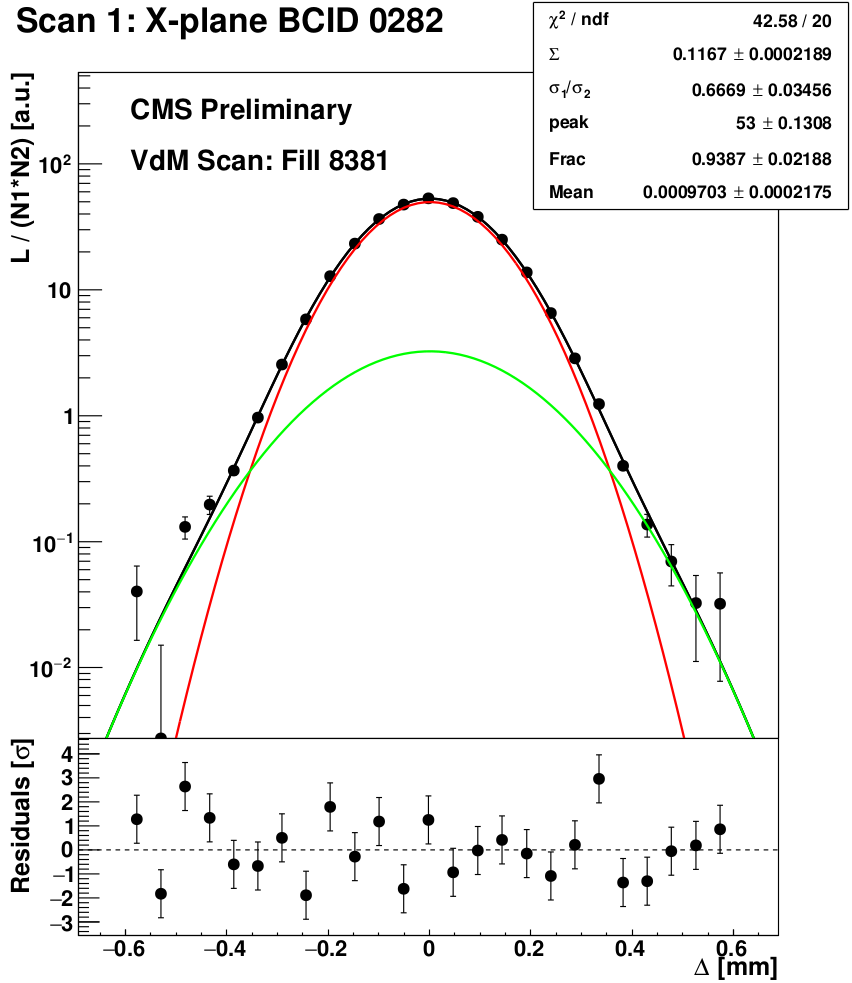
\includegraphics[width=.37\textwidth]{Chapter4/xscan.png}
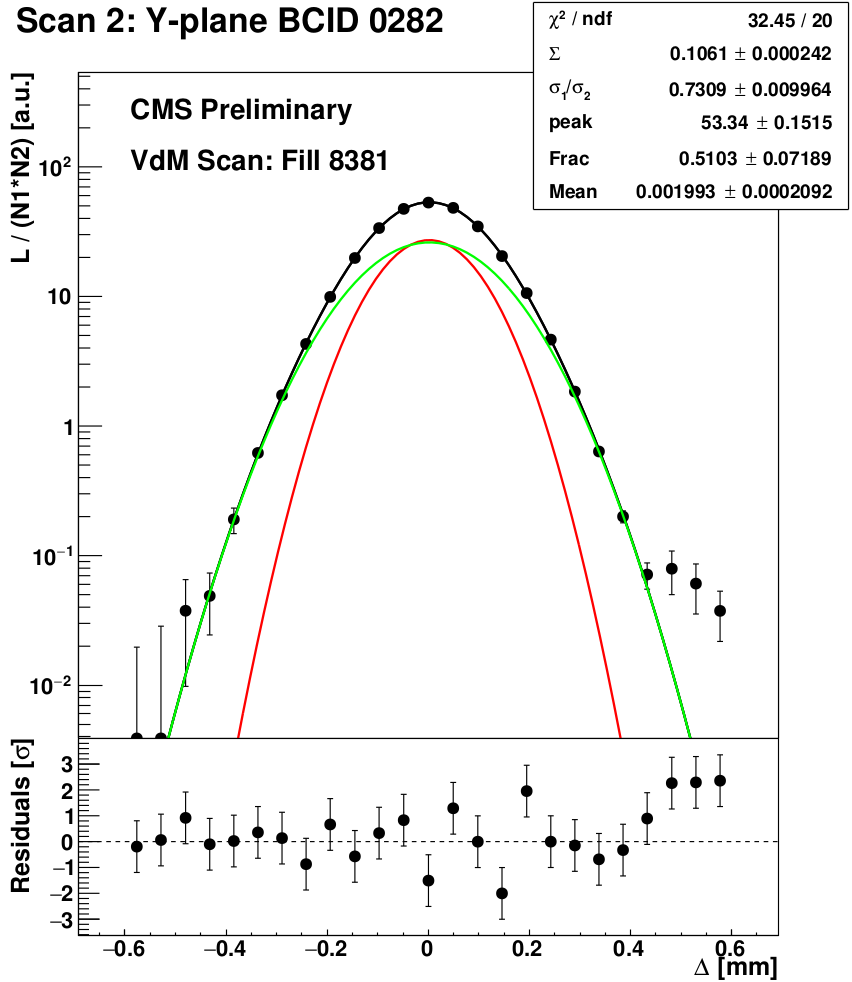
\includegraphics[width=.37\textwidth]{Chapter4/yscan.png}\\
\caption[vdM1 BCID 282]{Normalized rates and the resulting fitted curves with the DG+Const fit model as a function of the beam separation ($\Delta$) for BCID 282 for X (left) and Y (right) scan for the first vdM scan.}
\label{vdM1_282_XYscan}
\end{figure}
\end{center}

\newpage
For the remaining BCID's, the fits for both vdM and BI scans exhibit a very similar behavior, and in all cases, the fits have converged successfully. To evaluate the goodness of fit, Fig. \ref{chi2/ndof} displays a plot of the chi2/ndof for all the five scan pairs, which has a mean value of 1.88.
To compute $\sigma_{vis}$, the CapSigma $\Sigma_{x,y}$ and peak values have been extracted from the fits. Fig. \ref{capsigma_peak} presents the $\Sigma_{x,y}$ and peak values for all scan pairs. The plot clearly illustrates that both values reflect the fact that beam size increased over time in the $x$ dimension and decreased over time in the $y$ dimension.

\begin{center}
  \begin{figure}[h!]
    \centering
    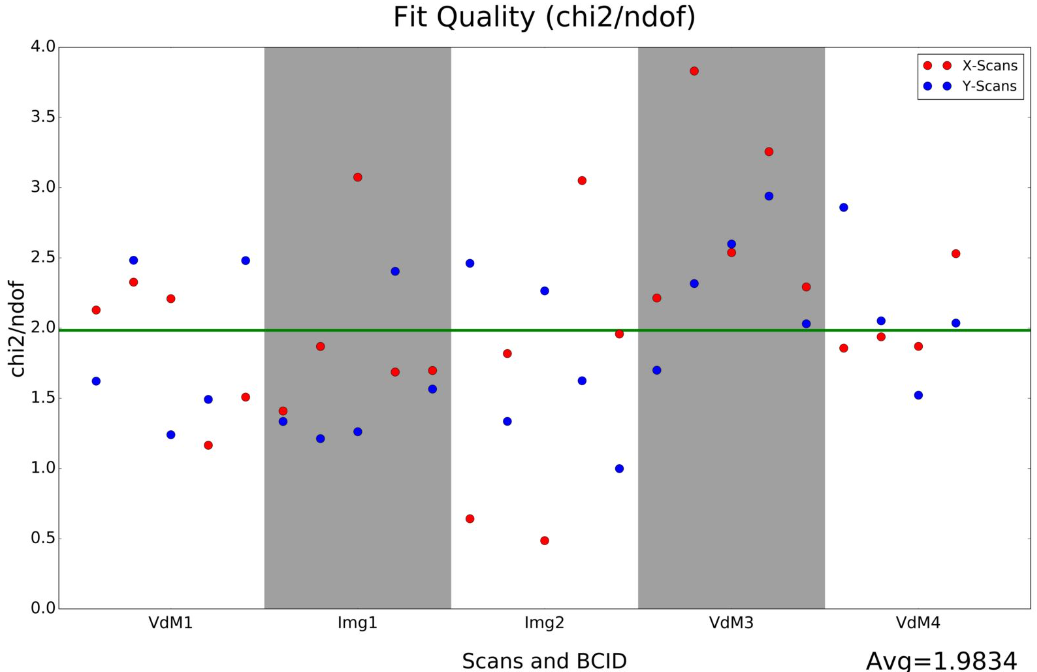
\includegraphics[scale=.03]{Chapter4/DGConst_chi2.png}
    \caption[chi2/ndof for all scan pairs]{ chi2/ndof for all the scan pairs.  where the red dots represent the X scans, and the blue dots represent the Y scans. It is important to note that in each scan, the BCIDs follow the same order, which is 282, 822, 2944, 3123, and 3302.} 
    \label{chi2/ndof}
  \end{figure}
\end{center}

\begin{center}
  \begin{figure}[h!]
    \centering
    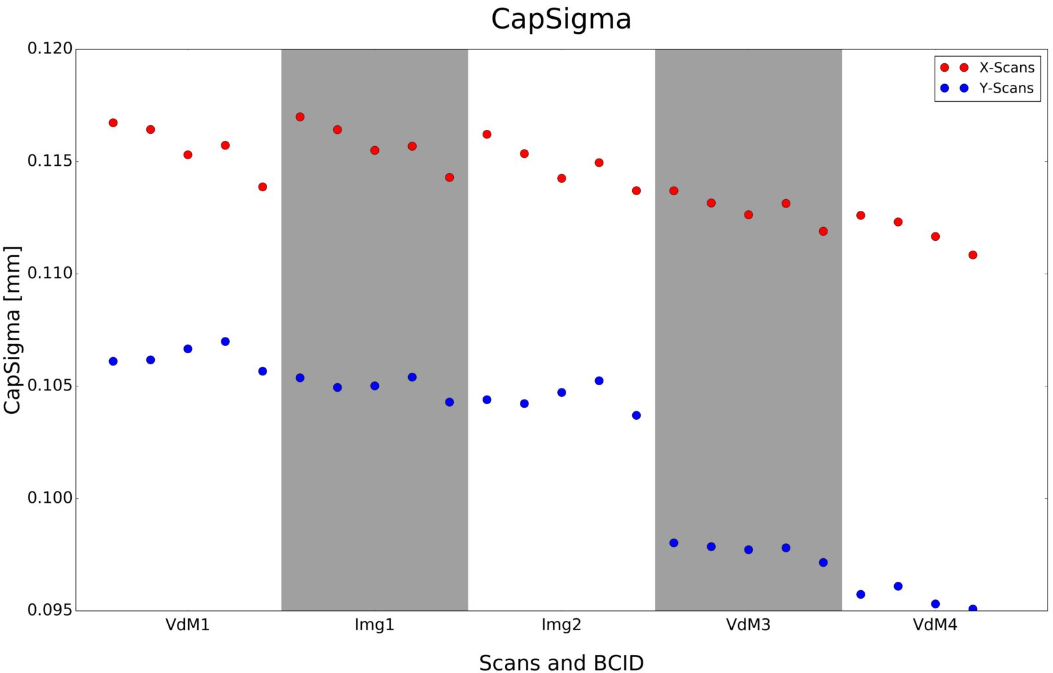
\includegraphics[width=.49\textwidth]{Chapter4/DGConst_CapSigma.png}
    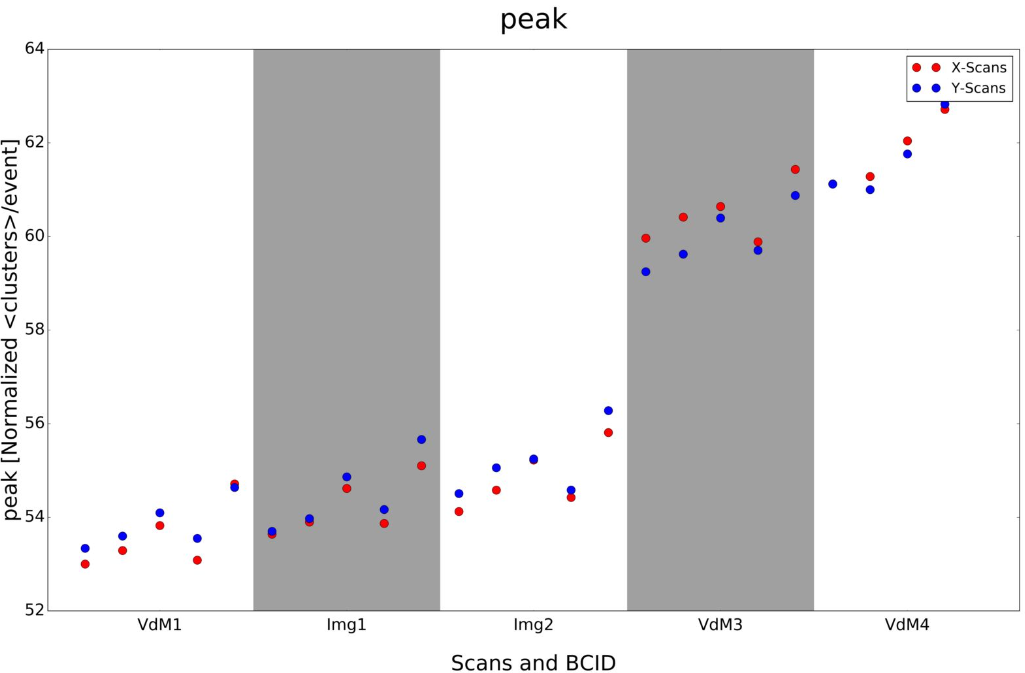
\includegraphics[width=.48\textwidth]{Chapter4/DGConst_peak.png}
    \caption[$\Sigma_{x,y}$ and peak values for all scan pairs]{$\Sigma_{x,y}$ (left) and Peak values (right) extracted from the fitted graph to compute $\sigma_{vis}$, where the red dots represent the X scans, and the blue dots represent the Y scans, note that in each scan, the BCIDs follow the same order, which is 282, 822, 2944, 3123, and 3302.} 
    \label{capsigma_peak}
  \end{figure}
\end{center}

The sigma visibe $\sigma_{vis}$ for all BCID's (vdM a BI acans) is computed from the fit results parameters Capital sigma $\Sigma_{x,y}$ and $peak_{x,y}$, this is done using the equation \ref{sigmavis_eq}. The value of $R(0,0)$ is obtained by taking the average of the peaks in the x and y directions ($R(0,0)=(Peak_{x}+Peak_{y})/2$), which have already been normalized, so \ref{sigmavis_eq} is rewritten as:

\begin{equation}
 \sigma_{vis}= 2\pi \Sigma_{x} \Sigma_{y} \Biggl( \frac{Peak_{x}+Peak_{y}}{2} \Biggl)
 \end{equation}
 
Fig \ref{sigmavis_perbcid} shows the  value of sigma visible $\sigma_{vis}$ per BCID for all the scans. where the error on $\sigma_{vis}$ is assigned as: 

\begin{equation}
\sigma_{vis\text{Err}}= 2 \pi \sqrt{ (\Sigma_{y} \cdot R \cdot \Sigma_{x\text{Err}})^{2} + (\Sigma_{x} \cdot R \cdot \Sigma_{y \text{Err}})^{2} + (\Sigma_{x} \Sigma_{y} R_{\text{Err}})^{2} }
\end{equation}

\begin{center}
  \begin{figure}[h!]
    \centering
    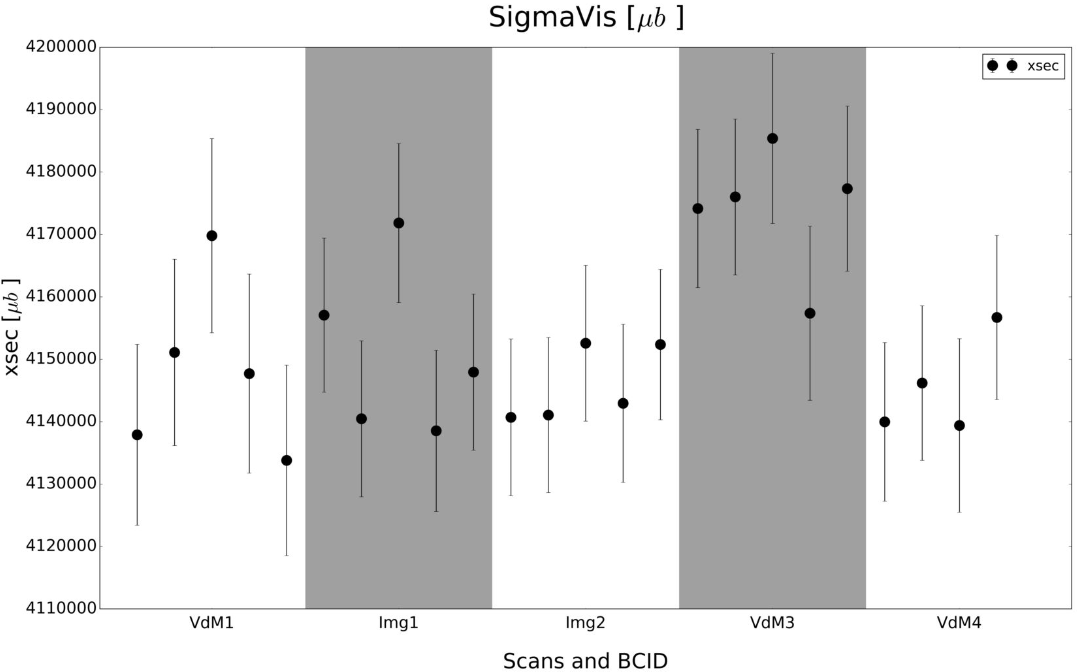
\includegraphics[scale=.25]{Chapter4/DGConst_xsec.png}
    \caption[$\sigma_{vis}$ per BCID for all scans]{ $\sigma_{vis}$ per BCID for all the scans,  in each scan, the BCID's follow the same order, which is 282, 822, 2944, 3123, and 3302.}
    \label{sigmavis_perbcid}
  \end{figure}
\end{center}


Fig \ref{sigmavis_perscan} shows the final  $\sigma_{vis}$ per Scan, which corresponds to the weighted average of the five BCIDs with the weight as: 

\begin{eqnarray}
\frac{1}{\sigma_{vis\text{Err}}^{2}}  \text{     where the error is     } \frac{1}{\sqrt{\sum \frac{1}{\sigma_{vis\text{Err}}^{2}}}}
\label{error}
\end{eqnarray}

After averaging the values of $\sigma_{vis}$ per scan, the error is assigned in the same manner as described in equation (\ref{error}). Figures \ref{sigmavis_perscan} and \ref{sigmavis_perbcid} illustrate that there is a systematic variation in $\sigma_{vis}$ between scans. To account for this, a systematic error is assigned as follows:

\begin{equation}
\sqrt{RMS^{2}-stat^{2}}
\end{equation}

Obtaining a final sigma visible for the calibration $\sigma_{vis}=4163 \pm 3 \text{(stat.)} \pm 12 \text{(syst.)} \text{ mb}$. This result will be useful for a precise luminosity measurement analysis for Run 3 in the CMS experiment of LHC.

\begin{center}
  \begin{figure}[ht]
    \centering
    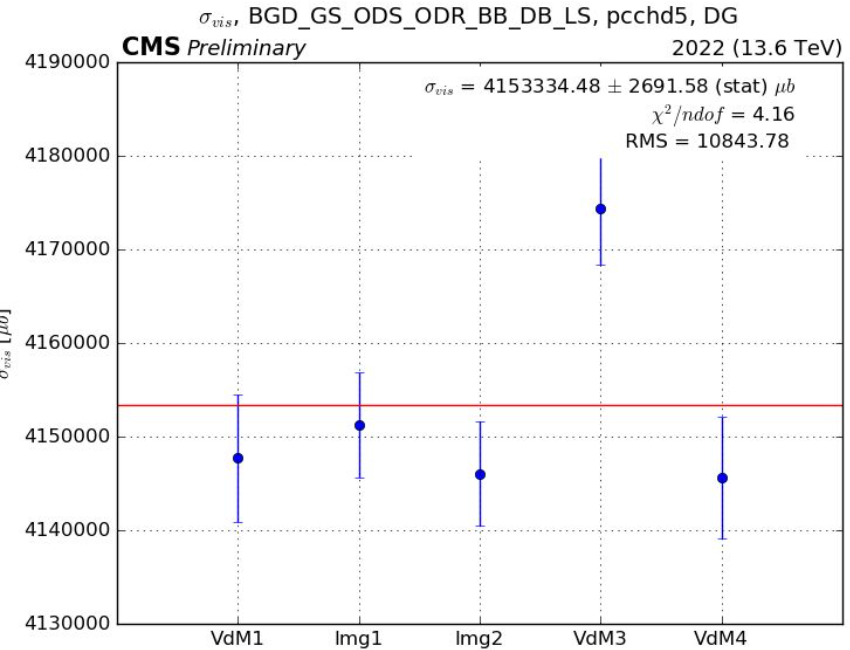
\includegraphics[scale=0.37]{Chapter4/xsec_perscan_v2.png}
    \caption[$\sigma_{vis}$ per Scan]{ $\sigma_{vis}$  per scan.} 
    \label{sigmavis_perscan}
  \end{figure}
\end{center}
